\section{Užívateľské požiadavky}

\subsection{Používateľské role}
Aplikácia bude rozlišovať následovné užívateľské role (zavedenie majiteľa nehnuteľnosti je motivovaný využívaním jednej inštancie aplikácie viacerými investormi):
\begin{itemize}
    \item \textbf{Nájomca} - môže vyhľadávať a rezervovať nehnuteľnosti, spravovať svoje rezervácie a recenzie po uskutočnení prenájmu.
    \item \textbf{Majiteľ nehnuteľnosti} - má plný prístup k funkciám pre správu svojich nehnuteľností, rezervácií a užívateľov a má možnosť reagovať na ich recenzie.
    \item \textbf{Administrátor} - má plný prístup k všetkým funkciám aplikácie, vrátane správy užívateľov a nehnuteľností a všetkých existujúcich recenzií.
\end{itemize}

\subsection{Funkcionality jednotlivých rolí}
Diagram používa značenie \textbf{CRUD} (create, read, update, delete) pre zobrazenie základných operácií, ktoré môže každá rola vykonávať nad entitami v systéme.
Pričom \textbf{CRU} znamená, že rola má právo vytvárať, čítať a aktualizovať danú entitu, ale nemá právo ju mazať.

\begin{figure}[!ht]\centering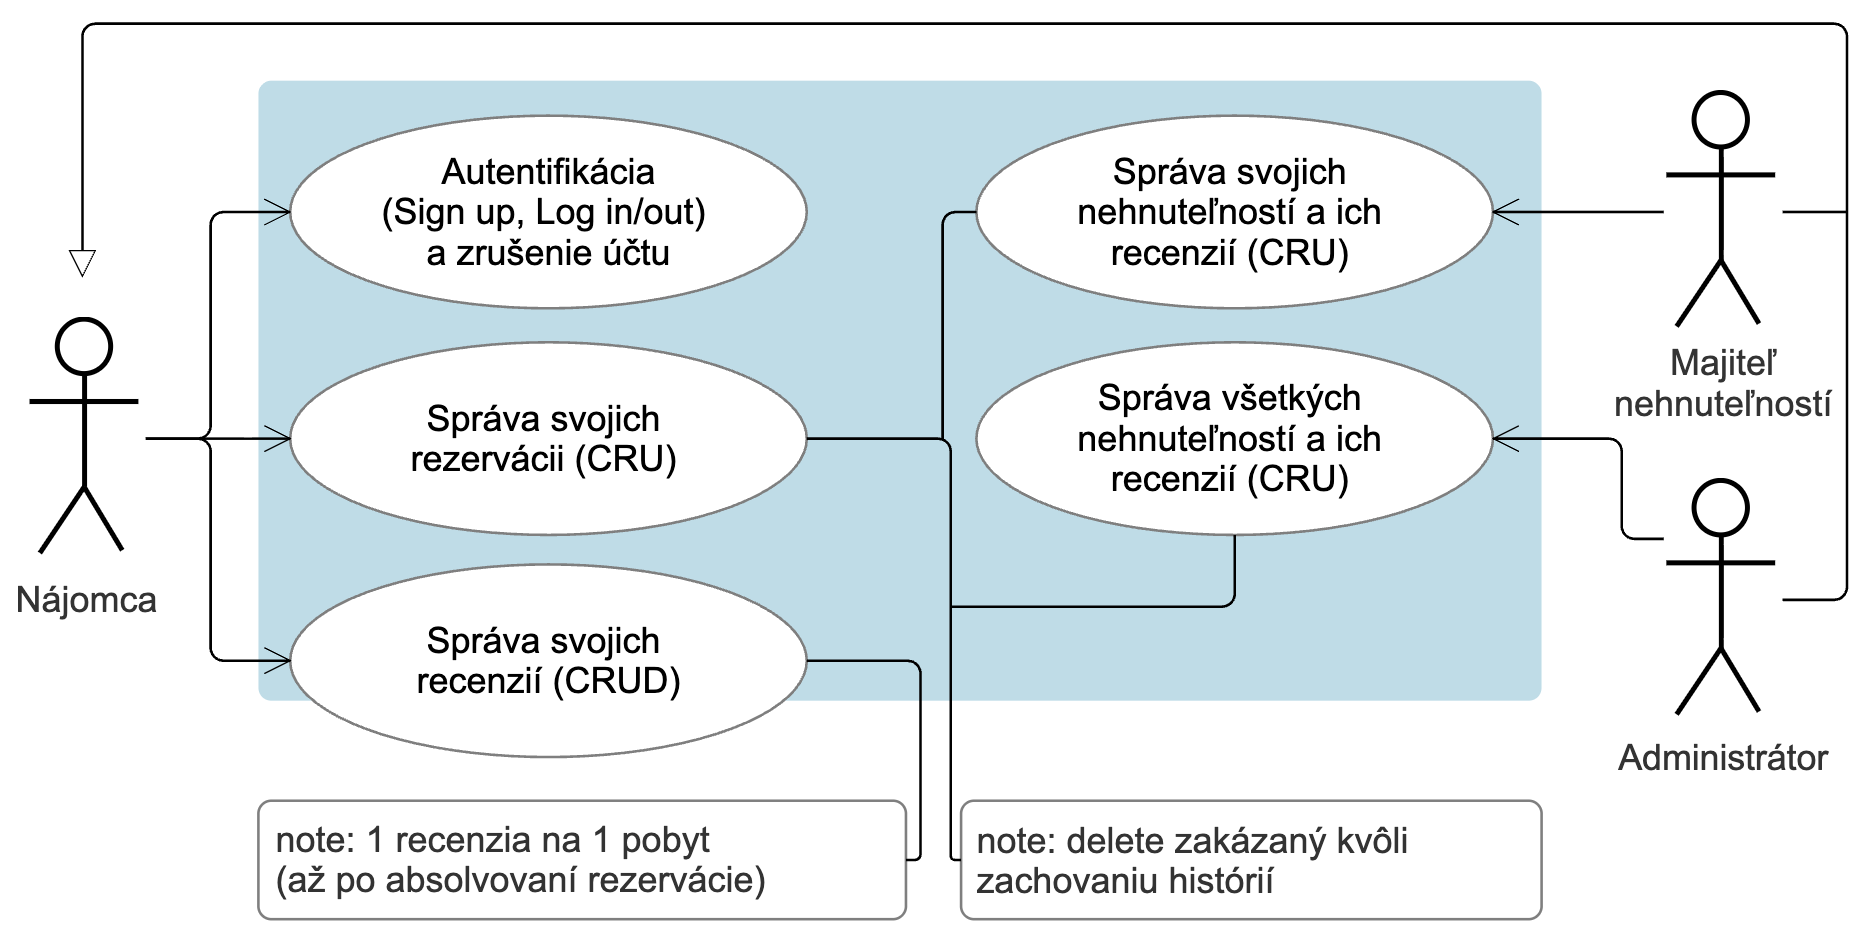
\includegraphics[width=\textwidth]{images/ur-uc.png}\end{figure}

Poznámky:
\begin{itemize}[itemsep=2pt]
    \item autentifikácia nie je hlavnou funkcionalitou, ale je zahrnutá pre zabezpečenie prístupu k funkciám aplikácie a teda je prerekvizitou pre využívanie ostatných funkcionalít,
    \item update (aktualizácia) môže byť obmedzená na určité atribúty záznamu v relačnej tabulke,
    \item delete (mazanie) musí byť obmedzené pre rezervácie, kvôli sledovaniu histórie (zrušenie rezervácie = aktualizácia, nie delete).
\end{itemize}

\subsection{Cesta užívateľa}
\subsubsection*{Nájomca}
Prihlási sa do aplikácie $\rightarrow$ prehliada si nehnuteľnosti $\rightarrow$ filtruje ich podľa svojich preferencií (lokácie, cena, vybavenie) $\rightarrow$ rezervuje vybranú nehnuteľnosť $\rightarrow$ spravuje svoje rezervácie (zobrazuje, aktualizuje, zruší) $\rightarrow$ vytvorí recenziu na nehnuteľnost po pobyte.

\subsubsection*{Majiteľ nehnuteľnosti}
Dedí od \textbf{Nájomca} a navyše: Prihlási sa do aplikácie $\rightarrow$ pridá nehnuteľnosť $\rightarrow$ spravuje svoje nehnuteľnosti (zobrazuje, aktualizuje, maže) $\rightarrow$ spravuje rezervácie (zobrazuje, aktualizuje, zruší) $\rightarrow$ reaguje na recenzie.

\subsubsection*{Administrátor}
Dedí od \textbf{Majiteľa nehnuteľnosti} a navyše: Prihlási sa do aplikácie $\rightarrow$ spravuje uživateľov, súbory, nehnuteľnosti, rezervácie a ich recenzie.
